\documentclass[20pt,a4paper]{report}
\usepackage[T2A,T1]{fontenc}
\usepackage[utf8]{inputenc}
\usepackage{blindtext}
\usepackage[russian]{babel}
\usepackage{mwe}
\usepackage{graphbox}
\usepackage[document]{ragged2e}
\usepackage[margin=50pt]{geometry}
\usepackage{longtable}
\usepackage{fontspec}
\usepackage{float}
\usepackage{titlesec}
\usepackage{setspace}
\usepackage{minted}

\usepackage{hyperref}
\hypersetup{
    colorlinks,
    citecolor=black,
    filecolor=black,
    linkcolor=black,
    urlcolor=black
}

\setstretch{1.5}
\graphicspath{{./images/}}
\setmainfont{LiberationSerif}
\setmonofont{Hack}
\titleformat{\chapter}{\normalfont\LARGE\bfseries}{\thechapter}{1em}{}
\titleclass{\chapter}{straight}
\titlespacing{\chapter}{0pt}{0pt}{5pt}[25pt]


\begin{document}
	\begin{titlepage}
		\begin{minipage}{0.3\textwidth}
		
\includegraphics[scale=0.03]{logo.png}	
		\end{minipage}
		\begin{minipage}{0.6\textwidth}\centering
			\textbf{
				Министерство науки и высшего образования Российской Федерации
				Федеральное государственное бюджетное образовательное 
				учреждение высшего образования
				«Московский государственный технический университет
				имени Н.Э. Баумана (национальный исследовательский университет)»
				(МГТУ им. Н.Э. Баумана)
			}	
		\end{minipage}
	
		\vspace{5cm}
		\centering
		\Large
		\textbf{
			Лабораторная работа №5 \\
			по курсу «Разработка интернет-приложений» \\
		}

		\vspace{6cm}
		\begin{flushright}
			Выполнил \\ 
			студент группы ИУ5-54Б \\ 
			Сысойкин Е.М. 
		\end{flushright}
		\vspace{5cm}
		Москва, 2020
	\end{titlepage}

	\chapter{Описание задания}
		\large
		\qquad Разработать макет сайта на языке разметки HTML, состоящий из нескольких связанных HTML-документов. Макет сайта должен включать следующие элементы: \\
		\begin{enumerate}
			\item Списки.
			\item Изображения.
			\item Таблицы.
			\item Фреймы, для создания меню используются гиперссылки.
			\item Плавающие фреймы.
			\item Элементы семантической разметки.
		\end{enumerate}

	\chapter{Текст программы}
		\qquad \textbf{index.html} \\
		\small
		\inputminted[tabsize=4, linenos]{html}{index.html}
		\large
		
		\qquad \textbf{content.html} \\
		\small
		\inputminted[tabsize=4, linenos]{html}{content.html}
		\large
		
		\qquad \textbf{images.html} \\
		\small
		\inputminted[tabsize=4, linenos]{html}{images.html}
		\large
		
		\qquad \textbf{lists.html} \\
		\small
		\inputminted[tabsize=4, linenos]{html}{lists.html}
		\large
		
		\qquad \textbf{table.html} \\
		\small
		\inputminted[tabsize=4, linenos]{html}{table.html}
		\large
		

	\chapter{Экранные формы}
		\begin{figure}[H]
			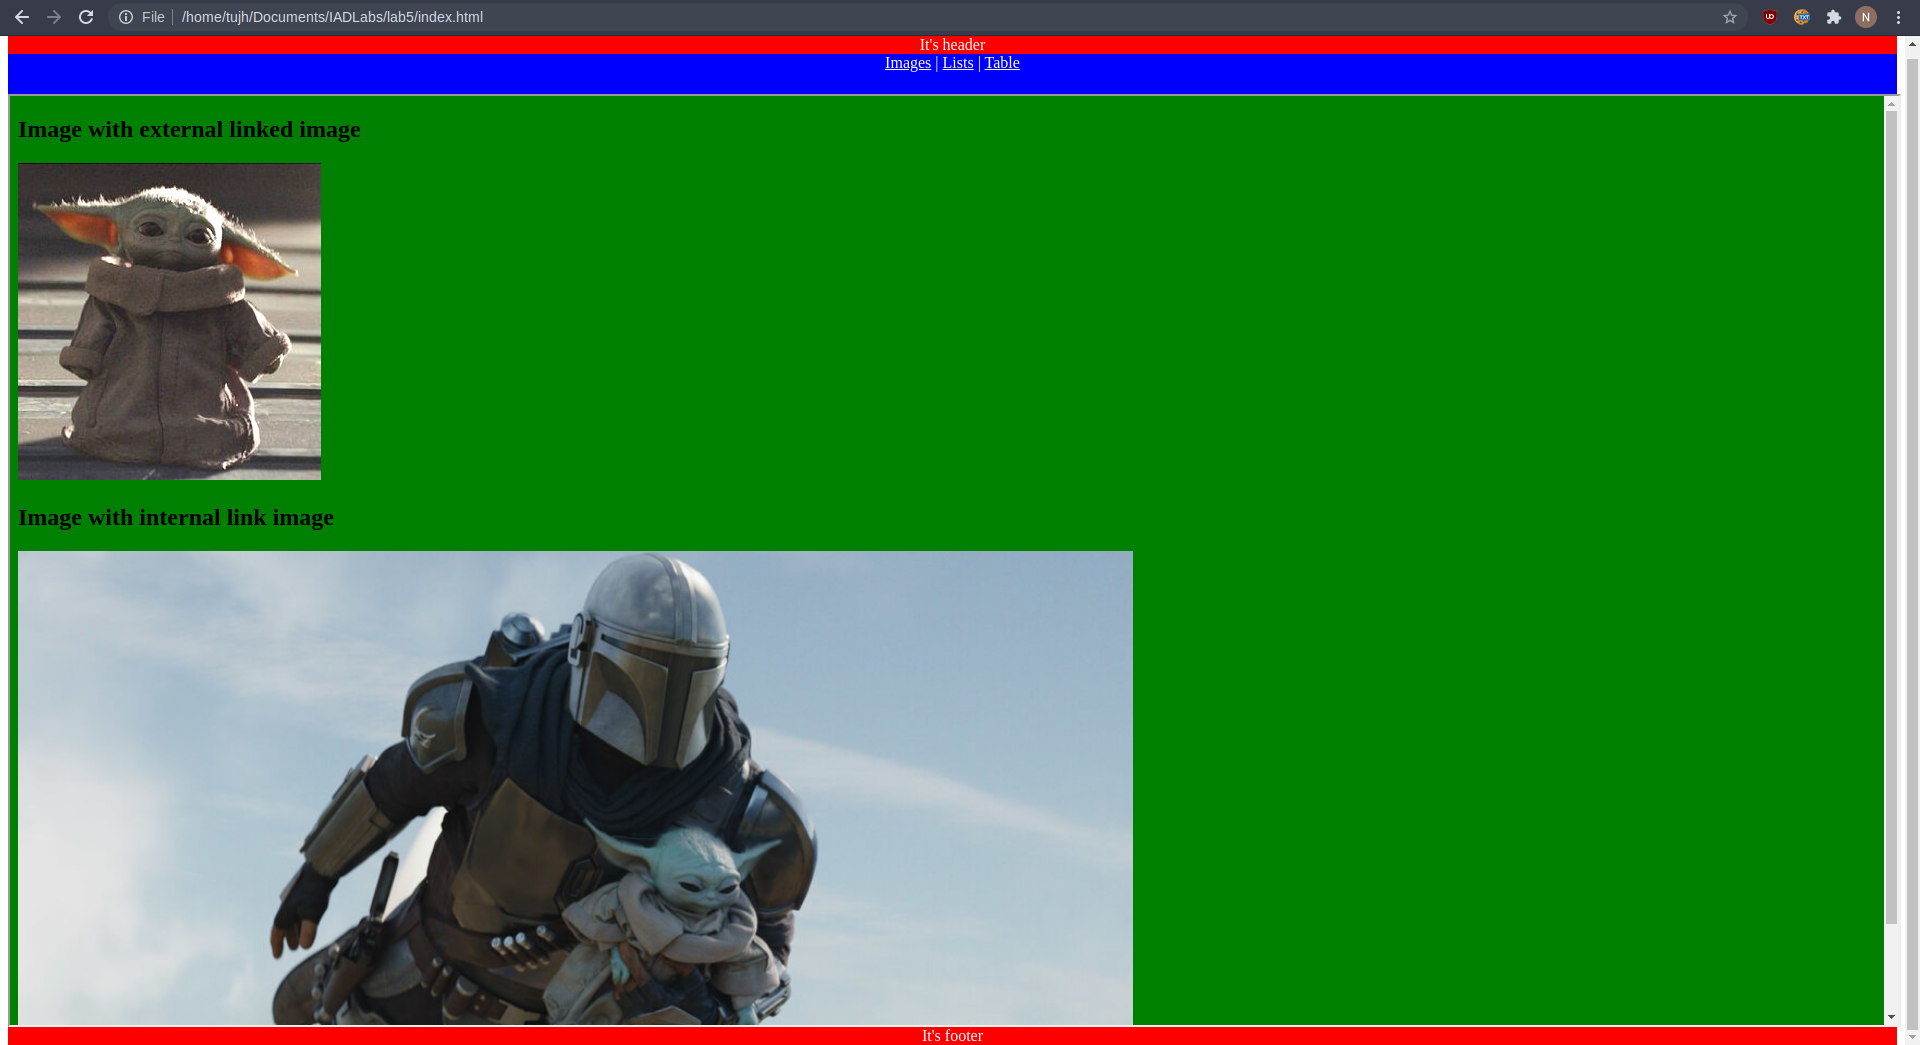
\includegraphics[width=\textwidth]{1.png}
		\end{figure}
		\begin{figure}[H]
			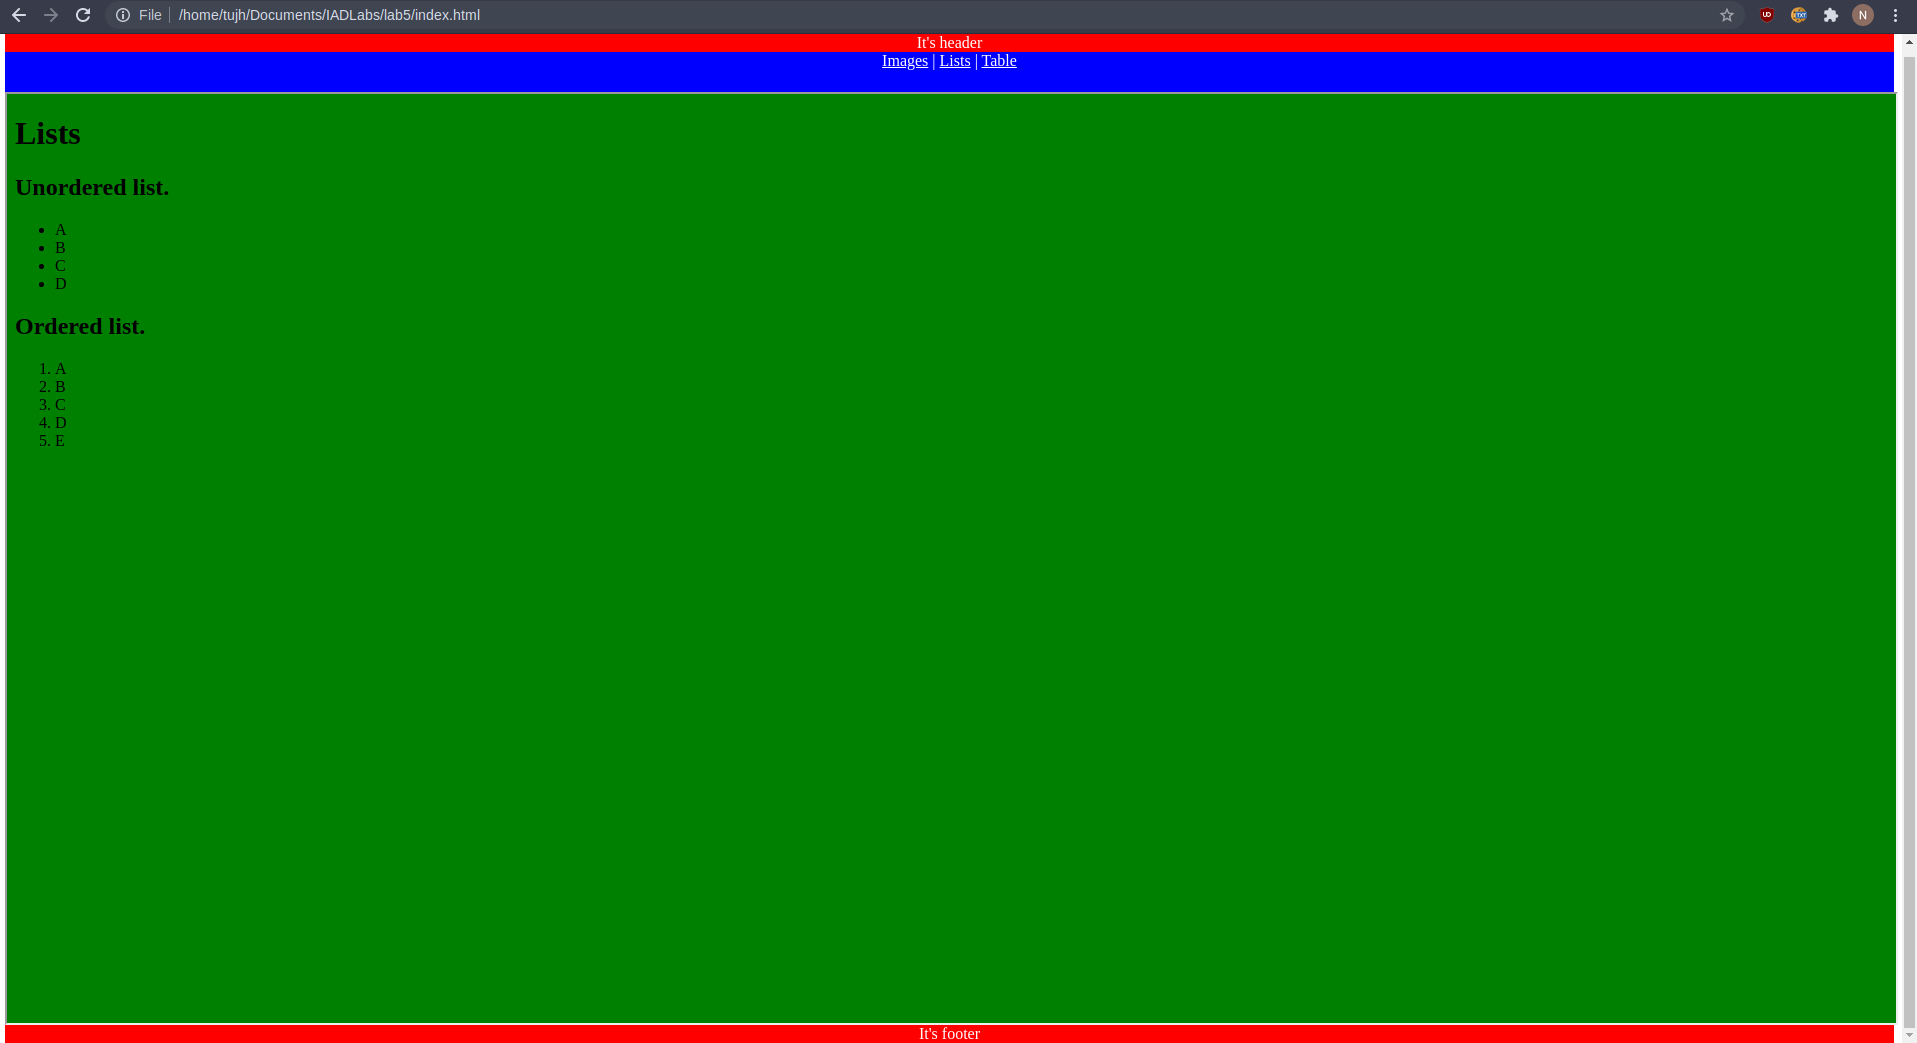
\includegraphics[width=\textwidth]{2.png}
		\end{figure}
		\begin{figure}[H]
			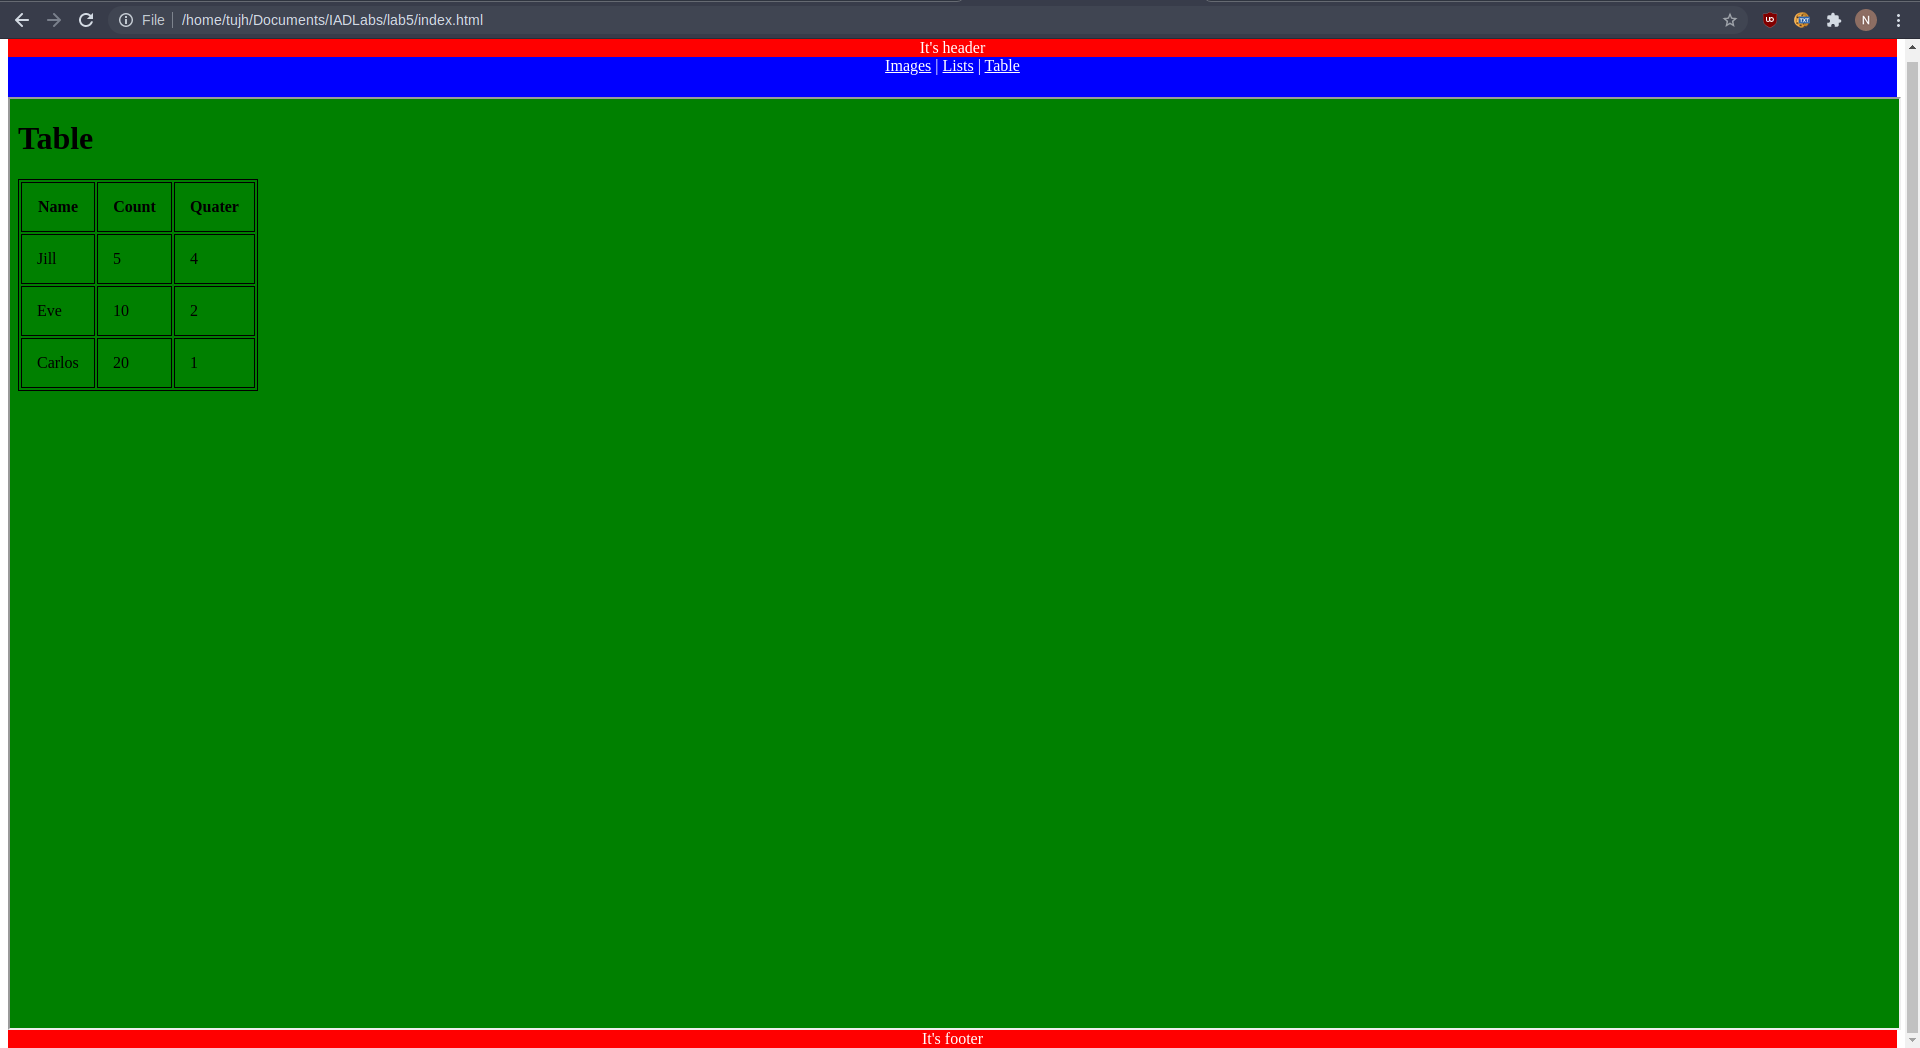
\includegraphics[width=\textwidth]{3.png}
		\end{figure}

\end{document}

